\ylDisplay{Vihmasadu} % Ülesande nimi
{Jaan Kalda} % Autor
{piirkonnavoor} % Voor
{2012} % Aasta
{G 7} % Ülesande nr.
{7} % Raskustase
{
% Teema: Varia
\ifStatement
Viilkatusega maja katus on peegelsümmeetriline: vertikaalne sümmeetriatasand on
ida-läänesuunaline ning katuse
põhja- ja lõunaküljed on omavahel risti. Mõlemal katusepoolel on vihmaveerenn,
mis kogub katusele langeva vee ning suunab selle tünni.
Sajab vihma ning puhub lõunatuul $u= \SI{6,0}{m/s}$; lõunaküljel paiknev tünn
täitub 2,0 korda kiiremini kui põhjaküljel paiknev tünn; võib
lugeda, et katuse läheduses piiskade langemissuund oluliselt ei muutu.
Milline on piiskade langemise keskmine kiirus (st kiiruse vertikaalkomponent)?
\fi


\ifHint
Horisontaalsuunalise tuule tõttu langevad vihmapiisad teatud nurga all vertikaali suhtes. Kuna lõunaküljel olev tünn täitub kaks korda kiiremini, siis lõunakatuse ristlõikepindala peab langevate piiskade risttasandis olema kaks korda suurem kui põhjaküljel.
\fi


\ifSolution
Tähistame katuse vertikaallõikel harja tähega $A$, räästad tähtedega $B$ ja $C$ ning lõigu $BC$ keskpunti tähega $O$. 
Täistame sümbolitega $s_1$, $s_2$ ja $s_3$ selliste piiskade trajektoorid, mis tabavad vastavalt põhjaräästast punktis $B$, harja punktis $A$ ning  lõunaräästast punktis $C$. Sirgete $s_1$ ja $s_2$ vahelisse ribasse jäävad piisad tabavad põhjakatust ning sirgete $s_2$ ja $s_3$ vahelisse ribasse jäävad 
piisad tabavad lõunakatust. Seega on veehulkade suhe võrdne ribade laiuste suhtega, mis omakorda on võrdne lõikude $BD$ ja $CD$ pikkuste suhtega, kus $D$ on sirge $s_2$ ja lõikepunkt lõiguga $BC$. Seetõttu $BD=\frac 13 BC$ ning järelikult $DO=BO-BD=\frac 16 BC$. Paneme tähele, et vihmapiiskade 
kiirusvektori horisontaal- ja vertikaalkomponentide suhe on võrdne lõikude $DO$ ja $OA=\frac 12 BC$ pikkuste suhtega; et $\frac {AO}{DO}=3$, siis piiskade 
langemise kiirus on $3u=\SI{18}{m/s}$.

\begin{center}
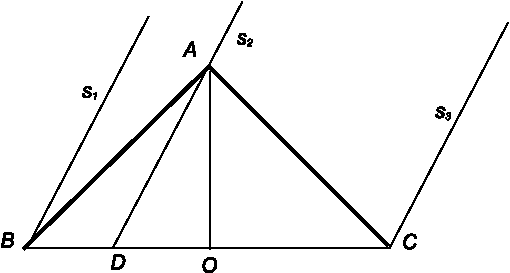
\includegraphics[width=0.5\linewidth]{2012-v2g-07-katus}
\end{center}
\fi


\ifEngStatement
% Problem name: Rain
A house has a mirror symmetric gable roof: the vertical plane of symmetry is East-West directional and the North and South sides of the roof are perpendicular to each other. At both sides of the roof there is a rainwater gutter that collects the water falling on the roof and directs it into a barrel. It is raining and South wind is blowing $u= \SI{6,0}{m/s}$. The barrel at the South side fills 2,0 times faster than the barrel at the North side. You can assume that the direction of the falling rain drops does not change significantly. What is the average speed of the falling drops (meaning the velocity’s vertical component)?
\fi


\ifEngHint
Because of the horizontally directed wind the rain drops fall down at a certain angle with respect to the vertical. Because the barrel at the South side fills two times faster then the cross-sectional area of the South roof on the perpendicular plane of the falling drops has to be two times bigger than on the North side.
\fi


\ifEngSolution
Let us mark the roof's ridge on the vertical cut as $A$, the eaves (the roof's bottom edges) as $B$ and $C$ and the center of the section $BC$ as $O$. With the symbols $s_1$, $s_2$ and $s_3$ let us mark the trajectories of such droplets that respectively hit the North eave at the point $B$, the ridge at the point $A$ and the South eave at the point $C$. The droplets staying on the strip between the lines $s_1$ and $s_2$ hit the North roof and the droplets staying on the strip between the lines $s_2$ and $s_3$ hit the South roof. Therefore the ratio of the water amounts is equal to the ratio of the widths of the strips which is in turn equal to the ratio of the lengths of the lines $BD$ and $CD$, where $D$ is the intersection point of the lines $s_2$ and $BC$. Because of this $BD=\frac 13 BC$ and therefore $DO=BO-BD=\frac 16 BC$. Let us notice that the ratio of the rain droplets' horizontal and vertical components is equal to the ratio of the lengths of the sections $DO$ and $OA=\frac 12 BC$; since $\frac {AO}{DO}=3$ then the falling speed of the droplets is $3u=\SI{18}{m/s}$.
\begin{center}
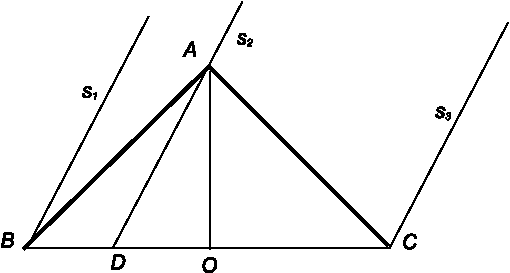
\includegraphics[width=0.5\linewidth]{2012-v2g-07-katus}
\end{center}
\fi
}